\documentclass[12pt]{article}
\usepackage{geometry}
\usepackage{graphicx}
\usepackage{array}
\usepackage{rotating}
\usepackage{pdflscape}
\usepackage{amsmath}
\usepackage{listings}
\numberwithin{figure}{section}
\numberwithin{table}{section}
\usepackage{float}
\usepackage{gensymb}

%border spacing
\geometry{
 a4paper,
 lmargin = 37mm,
 rmargin = 1in,
 tmargin = 1in,
 bmargin = 1in 
 }
 
%line spacing
\renewcommand{\baselinestretch}{1.5}  

\begin{document} 

\begin{titlepage}
\newgeometry{left=25mm}
\newcommand{\HRule}{\rule{\linewidth}{0.5mm}} % Defines a new command for the horizontal lines, change thickness here
\begin{figure}[H]
\centering

\includegraphics[scale=0.20]{logo}\\[1cm]
\end{figure}
\center 
{ \LARGE \bfseries Elephant Detection and Localization Using Infrasound}\\[1.5cm]
\Large Tharindu Prabhath Ranathunga\\
\Large Index No: 12001122\\[1cm]
\Large Supervisor: Dr Chamath Keppetiyagama\\[1cm]
\Large December 2016\\[1.5cm]
\large Submitted in partial fulfillment of the requirements of the B. Sc in Computer Science 4th year individual project\\[0.5cm] 

\includegraphics[scale=0.06]{ucsc}
\vfill % Fill the rest of the page with whitespace
\end{titlepage}
\pagenumbering{roman}
\section*{Declaration}
\paragraph{}
I certify that this dissertation does not incorporate, without acknowledgement, any material previously submitted for a degree or diploma in any university and to the best of my knowledge and belief, it does not contain any material previously published or written by another person or myself except where due reference is made in the text. I also hereby give consent for my dissertation, if accepted, be made available for photocopying and for interlibrary loans, and for the title and abstract to be made available to outside organizations.
\newpage
\section*{Preface}
\paragraph{}
This  document is the thesis for  the 4th Year Individual Project  for  partial  fulfillment  of  the requirements of the Degree of Bachelor of Science in Computer Science, at University of Colombo School of Computing, University of Colombo, Sri Lanka.

\paragraph{}
The intended audience of this document is the academic staff of the University Of Colombo School Of Computing and it is intended to enable them to determine whether the project should be approved as proposed, approved with modifications, or not approved.

\newpage
\tableofcontents


\newpage
\pagenumbering{arabic}
\newpage
\section{Introduction.}
\paragraph{}
The world elephant population has been on the decline \cite {13} due to many reasons, among which the human elephant conflict is a major cause. Human settlements and cultivations adjoining the forest areas have resulted in the blocking of elephant migration routes and further  the presence of crops attracts wild elephants, causing damages to livelihood of humans while threatening the lives of both elephants and humans. The wildlife conservation authorities worldwide do not possess an established method to manage this situation which is non-destructive to both elephants and humans, with most authorities having to resort to brute force, often consequently aggravating the situation in the long term \cite {13}. At present, the primary solution introduced is the use of electric fences around elephant habitats to prevent elephants venturing beyond their habitat to encroach into human settlements; an expensive and potentially life threatening solution.This effort is to address this problem in a sustainable way suitable for developing countries like Sri Lanka.
\subsection{Goal and objectives.}
\paragraph{}
The objective of this research is to implement  a cost effective input to a larger system that will help to solve the human elephant conflict building on and expanding upon the previous findings of related research. Research to date has found that elephants pass various messages using infra sound frequencies and this low frequency sound waves travel a greater distance than higher frequency waves  due to high frequency waves being more easily absorbed by air molecules compared to the lower frequency waves \cite {5}. In this research, an electronic system consisting of low cost sensors that have the capability of detecting infrasound calls emitted by the elephants as well as digital signal processing techniques are combined to  identify elephant  infrasonic vocalizations to localize the sound emitting sources. Further, attempts are made to use these information in various scenarios such as prior warning system before elephants enter a cultivation and elephant herd detection among other things.
\subsection{Human Elephant Conflict}
One of the major instigators of human elephant conflict is competition for space. In Africa and Asia, destruction of forests through logging, encroachment, slash-and-burn, shifting cultivation, and monoculture tree plantations are major threats to the survival of elephants \cite{28}. This occurs when elephants raid cultivations which are scattered over large area bounded with forests. In Sri Lanka, during 1999 to 2006 nearly 100 elephants were killed annually. 
\paragraph{}
This includes brief intro on HEC.
\subsection{Research question.} 
\paragraph{}
This research attempt to develop a method to distinguish an elephant call in a stream of sound data and to find an effective method of infrasound source localization using the phase difference of two infrasound waves captured by several sensors placed in different distances from the sound source. The research aims to answer two basic questions using a low cost sensor system consisting of off the shelf microphones capable of capturing infrasound:

\begin{enumerate}
\item How to identify an elephant call in an infrasound wave ? 
\item How to  localize a source emitting infrasound in a noisy environment ?
\end{enumerate}


\subsection{Background and Significance.} 

\paragraph{}
A typical human male voice in speech fluctuates around 110 Hertz, a female's voice at around 220 Hz and a child's at around 300 Hz. Among elephants, a typical male rumble fluctuates around a minimum of 12 Hz (more than 3 octaves below a man's voice), a female's rumble at around 13 Hz and a calf's around 22 Hz \cite {1} \cite {2}. In Asian elephants, this value fluctuates between 14 Hz to 24 Hz within 10 to 25 seconds \cite {3} due to their smaller vocal cords compared to African elephants.  Elephants produce a wide range  of sounds from very low frequency rumbles to higher frequency snorts, barks, roars, cries as well as many other type of  calls. 

\paragraph{}
Audio waves below 20 Hz frequency is considered as Infrasonic waves \cite {4}. As such, elephant rumbles can be considered as infrasonic waves and these rumbles follow all the properties of infrasonic waves. A significance of infrasonic waves is that it travels further than high frequency waves. Sound is a pressure wave vibration of molecules and as a result, whenever molecules move, there is an inevitable loss of energy as heat. As a result, sound is lost by heating the medium through which it propagates. Sound wave attenuation is frequency dependent in most media.

\begin{figure}[H]
\centering
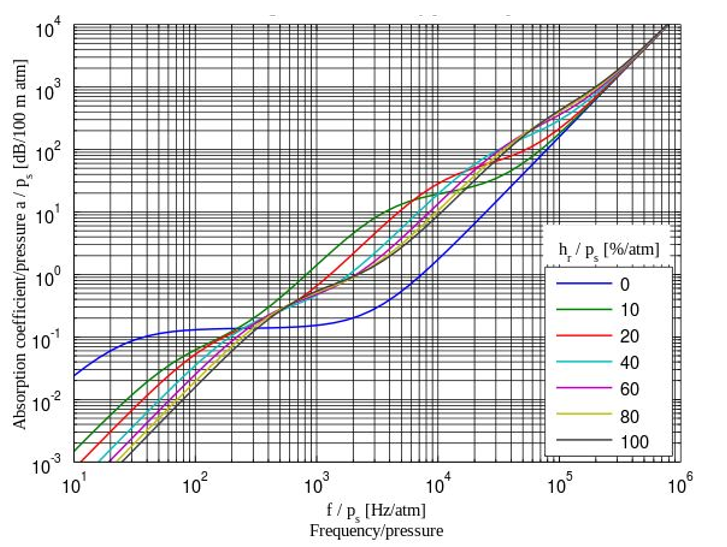
\includegraphics[width= 15cm]{a.png}
\caption{Sound absorption coefficient per atmosphere for air at 20 degree Celsius according to relative humidity per atmosphere.\cite{14}}
\label{fig:logo}
\end{figure}


\paragraph{}
The above image \ref{fig:logo} is a graph displaying the attenuation of sound at difference frequencies \cite {5}, which shows that low frequency waves have low absorption coefficient. Therefore, low frequencies are not absorbed well and travel further than high frequencies. This property of infrasound waves can be used  for the acoustic detection of the wave from a greater distance from the source of the sound. The low-frequency sounds used by elephants for long-range communication travel a distance that exceeds 1 km \cite {3}. As mentioned in the objectives, this research focusses on detecting elephant infrasonic calls from long distance and localizing them. Detecting and localizing elephants is an essential component of any viable solution to human elephant conflict. Attempts towards acoustic detection and localization of elephants exist in literature. However, due to high cost in infrasonic sensors and complexity in detection of these signals  in noisy environment, no system exists to date, that operation ready in the field.

\paragraph{}
Various types of devices which are capable of capturing infrasonic waves exist and they were mostly used for detecting geographical phenomena such as earthquakes and volcanic eruptions. One such device used by most related research is Infitec Infra 20, which has a sampling rate of 50Hz. This device can be considered as a low cost infra sound recorder compared to other existing devices and this costs US\$ 345 \cite {7}. A significance of the research is the attempt to use a laboratory made sensor system which cost only US\$ 15, which is capable of recording at a sampling rate of 44100 Hz. This sensor system consists of a Panasonic Omnidirectional Back Electret Condenser Microphone \cite{15} (Model WM-64C/WM-64K), LM358 IC for amplifying and a low pass filter\cite{16}.This sensor has the ability to capture infrasonic waves from a lower bound of 0 Hz to an approximate upper bound of 150 Hz.


\paragraph{}
The second research question is based on infrasound localization, which can be done by measuring physical quantities like sound pressure and particle velocity. The best localization technique which is used by nature (Animal sound localization) can be applied to this context in localizing a sound source digitally. Humans as well as most other land-living vertebrates use the time delay between the arrival of a sound wave at each ear to discern the direction of the source \cite {8}. Similarly, localization can be done digitally by calculating the inter-aural time delay  between two microphones lying on a specified distance, which will be further explained in the research methodology. Potential problems include the detection in noisy environment, sparsity and irregularity of elephant call and pattern recognition. These problems will be addressed using advanced digital signal processing techniques and the knowledge based on the existing literature.

\subsection{Scope of the thesis.}
\paragraph{}
As the final outcome, my intention is to introduce a low cost elephant detecting and localization system specialized for Asian countries using the sensor equipments made in the Sustainable Computing Research Group at University of Colombo School of Computing.

\begin{flushleft}
\text{This research attempts to:}
\end{flushleft}

\begin{itemize}

\item 	Identify an elephant call in the infrasound range with low latency.
\item 	Localizing an elephant call using the low cost sensors system consisting of a condenser microphone.
\end{itemize}

\newpage
\section{Review of Literature.}
\subsection{Elephant communication}
\paragraph{}
Various research types exist in this specific domain. The experiments carried out by Katharine Payne, a researcher in the Bio acoustics Research Program at the Laboratory of Ornithology at Cornell University, show that elephants use infrasound in communication, which can be considered as the initial steps of all research work on this area. In 1984, she discovered that elephants communicate in low frequencies during her research carried out at the Portland Zoo. Further, her work with William Langbauer, Jr. and Elizabeth Thomas have shown that elephants were indeed making infrasonic calls. Subsequent studies, in association with Joyce Poole, William Langbauer, Cynthia Moss, Russell Charif, Rowan Martin and others, took place in Kenya, Namibia, and Zimbabwe, leading to the conclusion that elephants use their powerful deep calls in long distance communication [6] and elephants make these calls when coordinating family and larger group behaviors, when competing for resources and dominance, as well as when attracting mates and announcing reproduction. Large vocal cords of elephants were able to produce low frequency sound signals considered as rumbles, which were able to travel around 5 km in distance \cite {6}. It is also revealed that the rumbles audible to human ears, are the harmonic waves created from the infrasonic fundamentals.


\paragraph{}
There has been comparatively less study of communication in Asian elephants. Acoustic communication in the Asian elephant by Dr. Shermin de Silva, a  James Smithson Fellow at Smithsonian Conservation Biology Institute, can be considered as a comprehensive study on communication in Asian elephants, which was published in the Behaviour biological journal in 2010. She categorized acoustic features into 8 'single' calls, 5 'combination' calls and one possibly unique male call, for a total of at least 14 distinct call types \cite {19}. Her observations and conclusions are based on the data collected at Udawalawa national park, Sri Lanka during 2007 and 2008. It is mentioned that 7 out of 14 distinct call types (rumble, rev, roar, cry, bark, grunt, husky-cry) are made out of elephants Larynx and most of the fundamentals of these calls were found to be infrasonic. While African elephants were the main subjects of considerable amount of existing literature with majority of these focusing on elephant detection in noisy environment; the human elephant conflict is more of a burning issue in South Asian countries like India and Sri Lanka.As a result, in 2002, there was an attempt at implementing a sensor system that detects infrasonic calls of elephants in Sri Lanka.

\paragraph{}
Elephant infrasound have not been recorded in wild Asian elephants anywhere in Asia prior to this research project in Sri Lanka in 2002. The prototype introduced by the above research was able to supports four infrasound sensors and is capable of standard DSP functions such as archiving and filtering. Sound detection has a long history although it was not specified to elephant infrasound calls. Recent researches have shown that this is possible using a template based or feature based technique. Matched filter method where two spectrograms of the pattern template and the signal are directly mapped, is a straightforward mechanism for detecting a pattern in a signal. Although it was optimal when finding the occurrence of a template in a recorded signal, it is sub optimal in the presence of complex noise \cite {10}. Therefore, a novel spectro-temporal method for signal enhancement based on the structure tensor \cite {11} was introduced by a group of researchers at University of Vienna, Austria. 
\newpage
\subsection{Sound localization}
\paragraph{}
There are many works related to sound localization using microphones. Many techniques and algorithms have been introduced during past decades to detect the direction of sound emitting source. These are mainly based on the following three type of principles.
\begin{enumerate}
\item Time difference of arrival, where the systems measure the difference in time between the signals received by the microphones to localize the sound source.
\item Direction of arrival, where the phase difference between the signals is used to locate the sound source \cite {20}.
\item Energy based sound localization, where the energy of sound wave decreases when the sound wave propagates in the air. By measuring the sound energy at different sensor locations, one may localize the sound source \cite {21}
\end{enumerate}

\paragraph{}
The most significant techniques is the time delay estimation, due to its simplicity and accuracy \cite {22}. Several research works have compared the algorithms such as cross correlation method \cite {23}, phase transform \cite {24} and maximum likelihood estimator \cite {25} used to estimate the time delay. There are instances where they have used two sensors or array of sensors for the localization, where; when number of sensors increases, the mean error generated becomes relatively low \cite {26}.

\paragraph{}
Results of the experiments in the form of simulation results \cite {26} show that all methods were able to estimate the time delay, where the peak position indicates the time delay estimation. However, the phase transformation method (PHAT) achieved a sharper peak than the other methods, which helps to estimate the real delay time more accurately in the real situation. The maximum likelihood method also achieved a sharp peak. Although cross correlation has the widest peak, it still can estimate the real time delay in the simulation conditions. Since these works can be directly incorporated to elephant call localization, we can guarantee that the accuracy of the localization results can be increased. As a result, we are able to select and use the most convenient and easily implemented method for the localization experiments. The environment of the localization scenario can result in the lagging of sound waves. As elephant localization is done in a forest environment, this is a factor that should be taken in to account. Many works have been done regarding the localization of sound in reverberation environment. The precedence effect describes the phenomenon, whereby echoes are spatially fused to the location of an initial sound, by selectively suppressing the directional information of lagging sounds (echo suppression). Echo suppression is a prerequisite for faithful sound localization in natural environments but its reliability depends on the behavioral context \cite {27}. These works can be integrated with our findings to be produce an accurate infrasonic localization. 

\subsection{Acoustic detection of elephants}
\paragraph{}
Although different literature exists with regard to acoustic detection of elephants and infrasound waves, there is no significant attempt towards an economically feasible solution for localizing Asian elephants through the use of infrasound calls, applicable to developing countries like Sri Lanka and India. The review will emphasize the importance towards a research on addressing the above problem.

\newpage
\subsection{Signal classification}

Related works on :
\begin{itemize}
  \item Biological researches on elephant communication. 
  \item Behavior of infra sound waves.
  \item Sound localization.
  \item Signal classification.
  \item Acoustic detection of elephants.
  \item Infra sound recording devices
\end{itemize}

\newpage
\section{Design and Methodology.}
\paragraph{}
As mentioned in the background, this research will not produce an ultimate machinery to detect and  localize elephants. Rather, it will be an input to a system of this calibre, which will increase the accuracy and also help validate the results of such a system. This research was undertaken in two steps to answer our two research questions.

\paragraph{}
The first phase of the research was mainly focused on the infra sound localization from a relatively large distance and the second phase was acoustic detection of elephants by processing the sounds recorded using the laboratory made sensors. In this chapter, the designs and the methods that we used to solve our two research questions is explained in detail. The process of the experiments related to infrasonic localization and detection of elephant calls is to be discussed later in this section.

Diagram of the whole system.


\subsection{Hardware used}

\paragraph{}
One of the objective of this research is to used low cost sustainable hardware. In this we present brief introductions on each commodity hardware used and the newly build and engineered hardware by us which will be used in the final outcome and in experiments. 

\paragraph{}
Since we ware dealing with infrasound we needed to have a device that is capable of recording infra sound upto 300Hz, which is the upper limit of an elephant call. Although they emit fundamentals at 5Hz-20Hz we needed to record their harmonics to identify the temporal structure of the calls clearly. We have used commodity infrasonic recorder initially and due to it's high cost in large scale deployment scenarios we have build a recording module using off the shelf microphones. In section 3.1.1 and 3.2.2 we compare and contrast these devices. 

\subsubsection{Infiltec INFRA-20}  

\paragraph{}
Researchers studying lightning activities in the atmosphere and seismic activities also use infrasonic detectors of
various forms. While the devices they use vary in a wide price range, the cheapest device we could identify in the market
is the Infiltec Model INFRA-20 \cite{29}. It costs about USD 300 which is still a significant cost when considering large
scale deployments. It has a sample rate of 50 and a precision of 16 bits. This can be powered by either house current 110-240 VAC or 12 VDC car battery. \cite{29}

\paragraph{}
The INFRA20 electronic noise level is about 20 counts (20 mPa or 60 dB SPL) over the full bandwidth, and this can be measured by cross connecting the ports on the internal differential pressure sensor. The lowest ambient infrasound level over the full bandwidth that you can expect to record with the INFRA20 is about 30 counts (30 mPa or 63.5 dB SPL), typically during the middle of the night when the wind is calm and there are no nearby infrasound sources. The INFRA20 background noise level is low enough so that the microbarom peak at about 0.2 Hz can sometimes be detected above the ambient noise when the wind is calm. \cite {29}. The following image is a INFRA20 unit.

\begin{figure}[H]
\centering
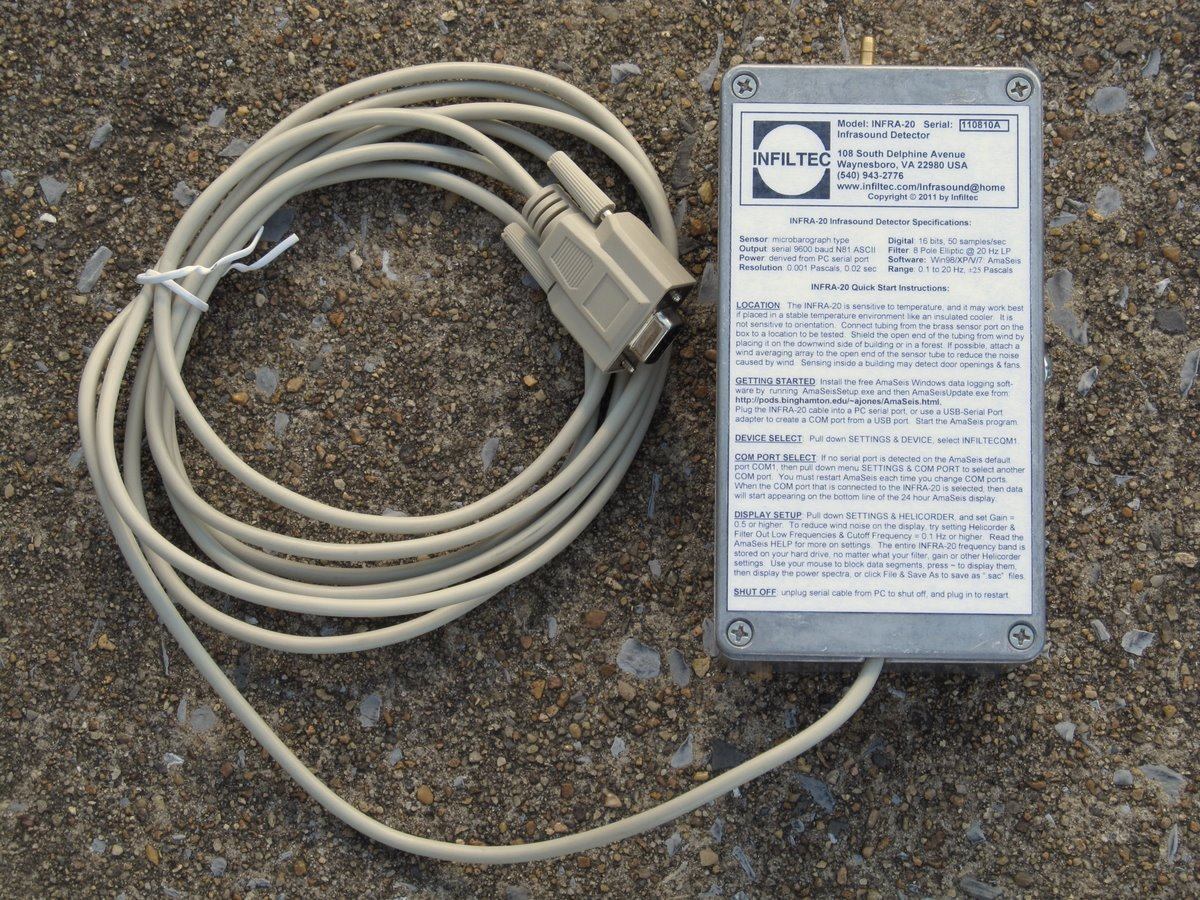
\includegraphics[width=10cm,height=13cm,keepaspectratio]{INFRA_20.jpg}
\caption{Infiltec INFRA-20 device}
\label{d:p12}
\end{figure}


\newpage
\subsubsection{Elocate sensors}

\paragraph{}
In order to localize elephants using infrasonic emissions, it is necessary to have cost effective infrasonic detector systems. Most importantly, since we are deploying them in rural areas of Country in large numbers, they need to have a cheap unit cost. Moreover, they should be able to run with minimum maintenance due to the unavailability of technical experts in potential deployment areas. The ability for a rural villager with minimum technical knowledge to set up and run such an elephant localization system in the neighborhood to protect their premises would be a great advantage. The system has to be non-invasive to the elephants to avoid legal barriers of deploying such a system by individuals living in affected areas.

\paragraph{}
To match our needs, we design and implement an infrasonic detector which we call Eloc node. The heart of an Eloc node is a Panasonic WM-61A omnidirectional back electret condenser microphone \cite{15}. Compared to ordinary condenser microphones, this microphone consumes less electric current and is therefore suitable for using in low power devices such as battery-operated embedded systems. An Eloc node consists of such a microphone and a small preamplifier circuitry connected to it inside a sealed plastic container.

\begin{figure}[H]
\centering
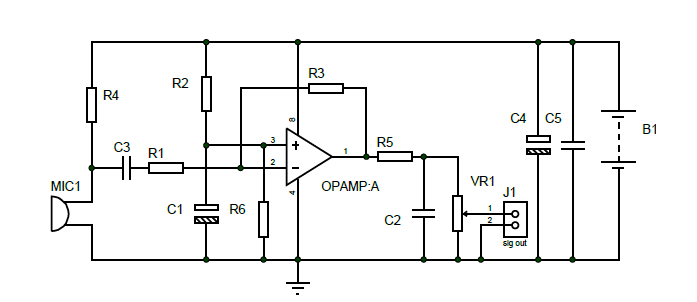
\includegraphics[width=10cm,height=13cm,keepaspectratio]{circuit.png}
\caption{The pre amplifier schematic used in an Eloc node.
It consists of an operational amplifier in inverting mode and
a low-pass filter. The low-pass filter attenuates frequencies
above 150 Hz.}
\label{image:circuit}
\end{figure}

\paragraph{}
As shown in Figure \ref{image:circuit} , the pre amplifier consists of an operational amplifier in inverting mode and a low-pass filter. The low-pass filter attenuates frequencies above 150 Hz since we are interested only in infrasonic frequency components. Eloc nodes get power from a 9V battery attached to the plastic container. This complete unit draws a current less than 50mA from the battery when the microphone is active. Hence, Eloc nodes could be powered by solar cells to avoid the need of replacing batteries once deployed in the field. The output of the Eloc nodes is an analog signal that we can sample directly using a suitable analog-to-digital converter before sending it over a wireless network for processing in the back-end. For the experimental purposes, we connect it directly to the audio input port of a computer for processing on-site.



\subsubsection{Subwoofer}

\subsubsection{Amplifier}


\newpage

\subsection{Localization}
\paragraph{}
Localization in this context is locating the infra sound emitting source. Localization of objects with tags which emit electromagnetic waves is a well studied problem with various localization techniques. Due to the maturity of such techniques,
the most obvious way of locating living objects such as humans and animals is tagging them with wireless devices. Radio collars placed on elephants is one good example of such an application \cite{32}. However, placing wireless devices on wild animals is intrusive to the natural behavior of the animals and such techniques are frowned upon by animal conversationalists. In addition, the difficulties in physically reaching elephants to attach these devices also makes this a cumbersome solution.

\paragraph{}
Our objective is to localize elephants by detecting their infrasonic emissions using Eloc nodes. Wang et al. have studied the use of acoustic sensor networks to passively localize wild animals \cite{33}. Our focus, is to use the infrasonic emissions from Asian elephants to detect and localize elephants. While many different sound localization methods are available in the literature, we use a simple technique based on time difference of arrival (TDOA) to locate infrasonic sources. The basis of this technique is presented by Kim et al. \cite{34} for localizing humans using the sounds they make. Due to the fact that those are audible sounds, their work considers capturing audible frequencies within close range mostly in indoor environments. In contrast, we consider a limited bandwidth in the infrasonic range which is heavily affected by natural low frequency noise sources such
as the wind. Reasons for using TDOA are it's implementation simplicity and ability to deploy in low powered computing devices. 

\subsubsection{Time delay estimation}
\paragraph{}
Time delay estimation is determined by the relative time difference of arrival between signals received by different sensors. Phase shift of each signal is measured relative to the other signal and this is used to calculate the time delay of arrival. This time delay is calculated using cross correlation technique which will be explained in the section below. In this scenario time delay estimation is done using the infrasonic signals received by  two Elocate sensors placed few distance away from each other. \ref{sinewave} will show how a sinusoid signal will be recorded by two Elcoate sensors. 

\begin{figure}[H]
\centering
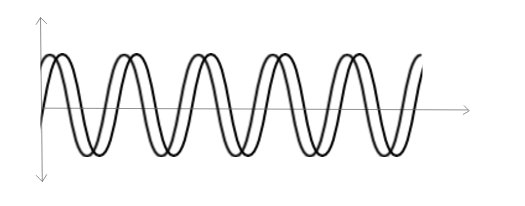
\includegraphics[width=100mm,height=50mm]{sinewave.png}
\caption{}
\label{sinewave}
\end{figure}

\paragraph{}
This time delay is used to used to calculate the angle between the sensors and the sound emitting source. And this can be used for the localization of the source. 

\subsubsection{Cross correlation}

\paragraph{}
Signal data recorded by two sensors is in the form of digital. Therefore these two signals are in the form of array having the normalized amplitude at each sample. Cross correlation come into play when we are calculating the time delay of arrival using these two arrays. Cross-correlation measure the similarity of two signals as a function of the displacement of one relative to the other. One signal recorded from one sensor is displaced relative to the other signal recorded from the remaining sensor and sliding inner product is taken. The below figure \ref{crosscor} show how one signal is slide relative to the other signal.

\begin{figure}[H]
\centering
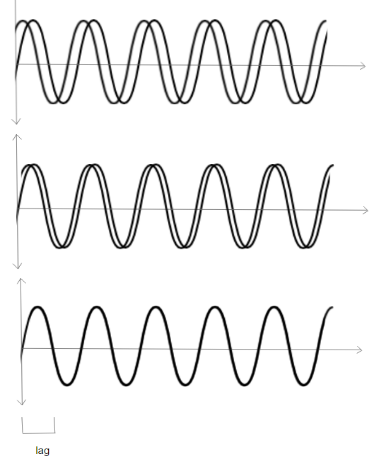
\includegraphics[width=80mm,height=150mm]{crosscor.png}
\caption{}
\label{crosscor}
\end{figure}

\paragraph{}
Slided amount along the time axis at the maximum sum of product gives the time delay of arrival. Because at the maximum sum of product gives where the signals correlate each other. Since these two signals are not identical and affected by different type of noise and other factors this maximum correlation gives a fair trade off for the time delay of arrival. One limitation of this method is that, since these signals are periodic, after the first maximum correlation, at each and every 180 degree shift an another maximum correlation occurs. Therefore the maximum time delay of arrival should not give a phase different more than 180 degree. This delay is depend on the distance between the two sensors and in infrasonic recording scenario this distance should be determined according to the signal wave length that we are going to localize. 

\paragraph{}
Asian elephants communication range is 14Hz to 24Hz \cite{2}. Since our Elocate nodes start cutting high frequencies at 150Hz maximum harmonic frequency of 20Hz fundamental is 120Hz. So we select 120Hz as the maximum record-able frequency. This selection enables us to use frequencies below 120 Hz for the localization which includes a number of higher harmonics in addition to the fundamental frequency components of the elephants in the infrasonic range. If we assume that the average temperature is 30 $^{\circ}$ Celcius velocity of the sound will be 350 m/s. So from equation (1).

\begin{equation}
v=f\lambda
\end{equation}
\begin{equation}
\lambda=v/f
\end{equation}
\begin{equation}
\lambda=350/120
\end{equation}
\begin{equation}
\lambda=2.916
\end{equation}

From the above calculation we select 3 meters as the distance between the Eloc nodes which is roughly the wavelength of the frequency 120 Hz under the atmospheric temperature of 30 $^{\circ}$ C to avoid capturing signals with a phase difference than 180 $^{\circ}$.


\subsubsection{Estimation of the sound direction}

\begin{figure}[H]
\centering
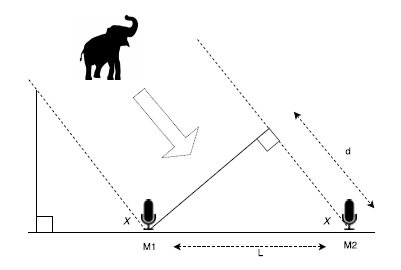
\includegraphics[width=140mm,height=100mm]{direction.png}
\caption{Basic setup to calculate the direction of an infrasonic
source using two Eloc nodes. The node pair is placed
within a constant distance to each other and continuously
capture data in a time synchronized manner in order to localize
the source using time difference of arrival.}
\label{direction}
\end{figure}

\paragraph{}
Figure \ref{direction} illustrates the basic setup to calculate the direction to an infrasonic source using two Eloc nodes. The infrasonic wavefront from the source arrives at the microphone M1 and then passes through it to the microphone M2. We take the distance the wavefront travel from M1 to M2 as d as illustrated in the figure and the time delay for this journey.is taken as D seconds. The same signal captured by M1 is captured by M2 after the D time delay. This time delay of arrival can be estimated by taking the cross correlation of the signals captured by M1 and M2. The lag towards the peak in the cross correlation graph indicates the phase shift between the two signals due to the delay D the infrasonic waves took to travel from the microphone M1 to the microphone M2. This phase shift can be measured as a number of samples, n. If the sampling rate at each microphone is f , we can have a representation of the time delay D as follows. 

\begin{equation}
D=n/f
\end{equation}

\paragraph{}
We can deduce an equation for the time delay D, according to the geometry in Figure \ref{direction}, as follows. The speed of
sound is taken as Vsound and the distance between the two microphones is L which are known values. The angle of infrasonic
waves arriving at the line connecting two microphones is x in degrees.

\begin{equation}
D = d/ Vsound = L Cos x/ Vsound
\end{equation}

\paragraph{}
Based on the Equations 5 and 6, we can calculate the angle x as follows.

\begin{equation}
x=\cos ^{ - 1} (nVsound/Lf)
\end{equation}

\paragraph{}
Equation 7 shows that when we know the sample lag between
the same sound captured by two Eloc nodes, we can
directly calculate the angle to the elephants location from the
node pair. However, when using a recorded sound clip as a
whole for the correlation calculation, different noise sources
that affected each Eloc node lower the accuracy of the final
result. To minimize such effects, we need multiple sound
clips from the elephant while it is in the same location over
the time period of capturing the sound. Due to the difficulty
of capturing multiple sound clips in such a way, we break a
single sound clip into windows so that we can consider each sample window as a separate data input for the correlation
calculation.

\begin{figure}[H]
\centering
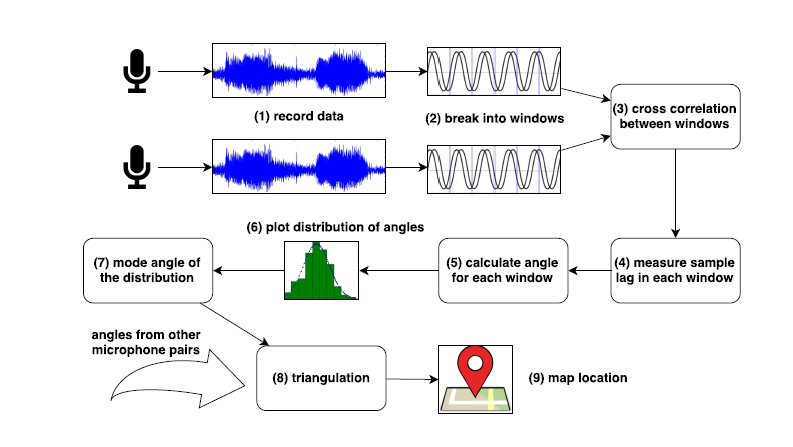
\includegraphics[width= \textwidth]{crosscor_implementation.png}
\caption{Process of calculating the location to an elephant.
A pair of Eloc nodes capture elephant sounds which we
break into windows, cross-correlate, calculated the sample
lag and finally use it as an input for the angle calculation.}
\label{crosscor_implementation}
\end{figure}

\paragraph{}
Figure \ref{crosscor_implementation} illustrates the complete process of locating an elephant using the infrasonic data. In the first step, two Eloc nodes capture infrasonic data in a time synchronized manner and we sample and quantize their output as the first step. Secondly, we break the data sets of the two channels into multiple windows of equal sizes to get multiple data samples from the original recordings. Then we take each corresponding window pair from the two channels and calculate
the cross correlation between them (Step 3). The number of sample points (i.e: lag) to the peak of the cross correlation
is the phase shift n in the Equation 7 that we compute in the fourth step. Using this value, we calculate the angle to the
infrasonic source for each sample window in Step 5.

\paragraph{}
Since we have multiple windows, we get multiple angles to the infrasonic source which may not necessarily be the
same value due to the noise in our recorded data. As Step 6 of Figure \ref{crosscor_implementation}, we plot the distribution of calculated angles for multiple windows for a known sound source. In the next step, we take the statistical mode of the distribution as the most representative angle that represents the actual angle towards the sound source. Our eventual goal is to deploy multiple pairs of Eloc nodes. In Step 8 we can then perform triangulation based on the angles calculated using each node pair to compute the position of the elephant in Step 9.

\paragraph{}
According to Equation 7 the angle calculation depends on the speed of sound, distance between the Eloc nodes, sampling
rate of the nodes, and the lag taken from the cross correlation. We can consider all the parameters as constants
except the lag, n, towards the cross correlation peak. The calculated angle is a non-linear function of n. That means, to
get the same change of degrees in the calculated angle, the required change in sample lag will be different from angle to
angle. Since this phenomena has an important effect on the errors we observed in real world experiments, we analyze the
behavior of angle calculation.

\subsubsection{Estimation of the error}

\paragraph{}
Minimum difference in the sample lag that we can measure depends on the sampling rate of the analogto-
digital conversion (ADC) on the connected computer. For a sampling rate of f , the minimum resolution of time measurement
we can have is (+/-)1= f . Since the sample lag n in Equation 7 has the same resolution, the error in n becomes
(+/-)1= f . We analyze the propagation of this error to the calculated angle as follows.

\paragraph{}
According to the error theory \cite{35}, the error, \Delta x, propagated to the calculated angle x is,

\begin{figure}[H]
\centering
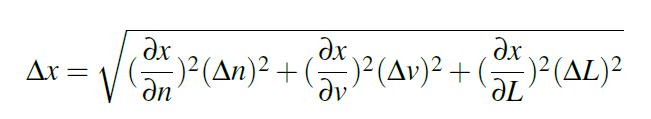
\includegraphics[width=100mm,height=20mm]{error.png}
\end{figure}

where, \Delta n, \Delta v, and \Delta L are the the measurement errors in the lag, speed of sound and the distance between Eloc nodes. Under the assumption that the speed of sound and the distance between the two Eloc are constants, this simplifies to,

\begin{figure}[H]
\centering
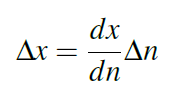
\includegraphics[width=30mm,height=15mm]{error1.png}
\end{figure}

\paragraph{}
From equation 7,

\begin{figure}[H]
\centering
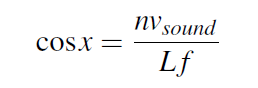
\includegraphics[width=35mm,height=15mm]{error2.png}
\end{figure}

\paragraph{}
We differentiate it by n,

\begin{figure}[H]
\centering
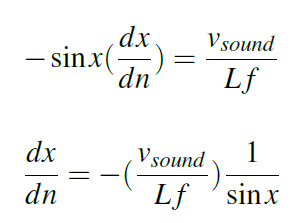
\includegraphics[width=45mm,height=35mm]{error3.png}
\end{figure}

\paragraph{}
During the time period of the experiments, we assume that the speed of sound (Vsound ), the distance between the two
microphones (L) and the sampling rate of the microphones ( f ) are constants. Therefore,

\begin{figure}[H]
\centering
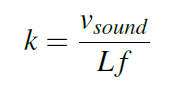
\includegraphics[width=30mm,height=15mm]{error4.png}
\end{figure}

\paragraph{}
So by substituting the constant,

\begin{equation}
\frac{dx}{dn}=-k(\frac{1}{sin x})
\end{equation}



\subsection{Acoustic detection}
Due to the fact that the elephants communicate with each other by low-frequency sounds, which travel distances of several kilometers acoustic detection of elephants by their calls has become a promising approach. In this section we discuss the methodology of automating the detection of recorded elephant calls in a machine learning approach. Major challenges that we faced in the process of automating the elephant call detection are the large variety of uncontrollable noises from wind, rain, cars and airplanes, and sparsity and irregularity of elephant calls, which makes it difficult to predict the occurrence of a call. We employ an image processing based signal filtering mechanism to filter out this noise based on the work of \cite{11}.

Initially, we train the model without any signal enhancement or noise filtering mechanism. And then the spectro temporal enchacment proposed by \cite{11} is applied and results are compared. We are dealing with a signal data set which basically are audio clips in time domain. The signal consist of the mean amplitude of each sample and all other information such as frequency and wavelength can be extracted using it. To a classifier these raw data doesn't make any sense. Main objective of this kind of classification is clearly distinguish the waves of elephant calls and waves without elephant calls. So that the all the features that distinguish elephant calls from other sounds should be extracted to feed into the classifier. So in the first step features are extracted from the waves.

\subsubsection{Feature extraction}
The first step in automatic elephant call detection is to extract features i.e. identify the components of the audio signals that are good for detecting the elephant vocal contents and discarding all the other stuff. Feature extraction is the process of computing a compact compact numerical representation that can be categorize a segment of audio. Naturally this done in human ears by filtering out according to the shape of the vocal tract including tongue, teeth etc. The same technique is modeled mathematically to filter out the unnecessary things mentioned above. 

\begin{figure}[H]
\centering
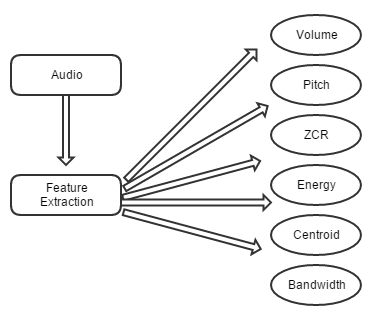
\includegraphics[width=12cm,height=15cm,keepaspectratio]{feature_extraction.png}
\caption{Overview of feature extraction.}
\label{feature_extraction}
\end{figure}




\subsubsection{Mel Frequency Cepstral Coefficients}
\subsubsection{Rumble detection}
\subsubsection{Signal enhancement}
\subsubsection{Classification using SVM}


\newpage
\section{Implementation.}
In this chapter we will be discussing on implementation process of the Elocate nodes, localization and automated acoustic detection system based on machine learning.
\subsection{Implementation of Elocate nodes}
\paragraph{}
Section 3.1.2 is consist of the architecture and design of the Elocate nodes and in here we will be discussing on the implementation constraints. 

\begin{figure}[H]
\centering
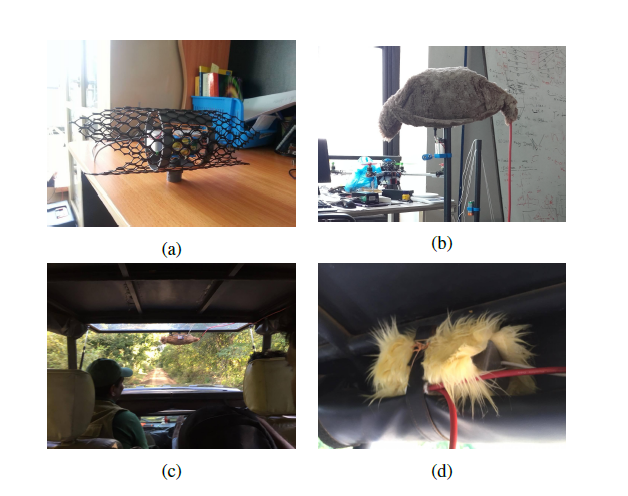
\includegraphics[width=12cm,height=15cm,keepaspectratio]{eloc_implementation.png}
\caption{(a) The microphone together with pre-amp circuitry
is placed inside a sealed plastic box and then placed
inside the wire-frame with shock mounting. (b) This wireframe
was covered with a soft material to cancel wind noise.
In (c) and (d), two of these microphones are mounted in the
front and back of a vehicle for field experiments.}
\label{figure:eloc}
\end{figure}

\paragraph{}
Since we are interested in low frequencies, the noise imposed by the wind plays an important role. Initial experiments indicated that the Eloc nodes are unable to detect low frequency sources since they are submerged under the wind noise floor. Therefore we design and built a wind barrier around the microphones to protect them from wind noise as shown in Figure \ref{figure:eloc}. This wind barrier consists of a wireframe with a soft material attached to it. An Eloc node is placed inside the wireframe using a vibration-proof mounting. We used different soft materials for the fur layer on the wireframe as well as several shapes for the wire frame to identify the most appropriate combination. The selected fur layer consists of a cheap artificial fur material we found off the shelf. Detailed comparison of the Eloc node with the INFRA20 will be on the Evaluation.


\subsection{Localization}

\subsubsection{Estimation of the direction}

\begin{figure}[H]
\centering
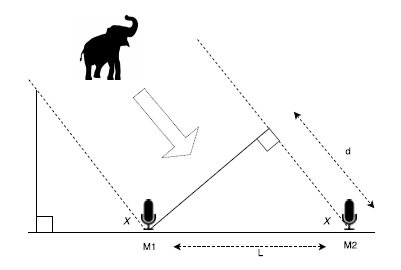
\includegraphics[width=100mm,height=80mm]{direction.png}
\label{direction1}
\end{figure}
\paragraph{}

This was implemented using Python and Matlab for different experiments and deployment environments. This estimation gives a angle , precisely a distribution of angles calculated in each window. Default windows size used is 10000 samples. At this phase the audio recorded is the input to the angle (x in the above diagram) calculation function with the parameters, distance between two Elocate nodes, sample rate and velocity of the sound. The audio should be a two channel audio consisting with data from two Elcoate nodes and recorded in 16 bit wave format because in the implementation audio is normalized by dividing every amplitude by the maximum value of 16 bit representation. A window from signal1 is cross-correlated with the corresponding window in signal2 and the lag is calculated. As mentioned in the Methodology this lag is then used to calculate the angle x in the above figure. This is done for each and every window and a angle calculated from each window is stored in an array. If an abnormal result is generated by the noise that values are simply neglected by dropping all the sine values greater than one. Following code snippet shows this implementation in Python.

\begin{lstlisting}
#filename , sampel rate, distance between two nodes, 
velocity of sound
def getAngle(fi,fs,d,vs):   
    fs, data = wavfile.read(fi)
    data=data.astype('float64')
    data=data.T/32767
    s1=data[0]
    s2=data[1]
    limit=len(data[0])
    fs = 44100
    start_window = 1
    end_window = 10000
    window = 10000
    total = 0
    arr=[]
    while(end_window<limit):
        s1=data[0][start_window:end_window]
        s2=data[1][start_window:end_window]
        xcor=np.correlate(s1,s2,'full')
        m=max(xcor)
        im=np.argmax(xcor)
        start_window = start_window + window
        end_window = end_window + window
        deference = abs(im - window)
        ang = deference*vs/fs/d
        if(ang<=1):
            angle=np.arcsin(ang)
            arr.append(math.degrees(angle))
    plt.hist(arr)
    plt.show()

    return(arr)
\end{lstlisting}

\paragraph{}
For importing wave files wavefile module from Scipy is used and Correlate from Numpy is used for cross-correlation. Matplotlib is used to visualize calculated angles for each window in a particular wave file in a histogram. 


\subsection{Pattern}
Data are in wave format. As the name suggest it consist of the raw wave information in the time domain. 
\subsection{Feature extraction}
\paragraph{}
Implementation of the feature extraction was done in Python. MFCC was used in the initial phase which is in Python speeches. Default frequency range of MFCC is shifted down where maximum frequency will be 300Hz which is suitable for elephant range.
\begin{lstlisting}
from python_speech_features import mfcc
from python_speech_features import logfbank
import scipy.io.wavfile as wav



def extract_features(wavefile,winlen):
    (rate,sig) = wav.read(wavefile)
    data=sig.T
    #checking the audio is dual channel or single
    if(len(data)==2):
        mfcc_feat = mfcc(data[0],rate,winlen,winstep=1,highfreq=300)
    else:
        mfcc_feat = mfcc(data.T,rate,winlen,winstep=1,highfreq=300)
        
    return mfcc_feat
\end{lstlisting}

\paragraph{}
This will return a feature vector consist of 13 features which described in the methodology. Length of a window can be parsed according to different scenarios.

\newpage
\subsection{Spectrogram visualization}
\begin{lstlisting}
#!/usr/bin/env python
#coding: utf-8
import numpy as np
from matplotlib import pyplot as plt
import scipy.io.wavfile as wav
from numpy.lib import stride_tricks

""" short time fourier transform of audio signal """
def stft(sig, frameSize, overlapFac=0.5, window=np.hanning):
    win = window(frameSize)
    hopSize = int(frameSize - np.floor(overlapFac * frameSize))
    
    # zeros at beginning (thus center of 1st window should be for sample nr. 0)
    samples = np.append(np.zeros(np.floor(frameSize/2.0)), sig)    
    # cols for windowing
    cols = np.ceil( (len(samples) - frameSize) / float(hopSize)) + 1
    # zeros at end (thus samples can be fully covered by frames)
    samples = np.append(samples, np.zeros(frameSize))
    
    frames = stride_tricks.as_strided(samples, shape=(cols, frameSize), strides=(samples.strides[0]*hopSize, samples.strides[0])).copy()
    frames *= win
    
    return np.fft.rfft(frames)    
    
""" scale frequency axis logarithmically """    
def logscale_spec(spec, sr=44100, factor=20.):
    timebins, freqbins = np.shape(spec)

    scale = np.linspace(0, 1, freqbins) ** factor
    scale *= (freqbins-1)/max(scale)
    scale = np.unique(np.round(scale))
    
    # create spectrogram with new freq bins
    newspec = np.complex128(np.zeros([timebins, len(scale)]))
    for i in range(0, len(scale)):
        if i == len(scale)-1:
            newspec[:,i] = np.sum(spec[:,scale[i]:], axis=1)
        else:        
            newspec[:,i] = np.sum(spec[:,scale[i]:scale[i+1]], axis=1)
    
    # list center freq of bins
    allfreqs = np.abs(np.fft.fftfreq(freqbins*2, 1./sr)[:freqbins+1])
    freqs = []
    for i in range(0, len(scale)):
        if i == len(scale)-1:
            freqs += [np.mean(allfreqs[scale[i]:])]
        else:
            freqs += [np.mean(allfreqs[scale[i]:scale[i+1]])]
    
    return newspec, freqs

""" plot spectrogram"""
def plotstft(audiopath, binsize=2**10, plotpath=None, colormap="jet"):
    samplerate, samples = wav.read(audiopath)
    s = stft(samples, binsize)
    
    sshow, freq = logscale_spec(s, factor=1.0, sr=samplerate)
    ims = 20.*np.log10(np.abs(sshow)/10e-6) # amplitude to decibel
    
    timebins, freqbins = np.shape(ims)
    
    plt.figure(figsize=(15, 7.5))
    plt.imshow(np.transpose(ims), origin="lower", aspect="auto", cmap=colormap, interpolation="none")
    plt.colorbar()

    plt.xlabel("time (s)")
    plt.ylabel("frequency (hz)")
    plt.xlim([0, timebins-1])
    plt.ylim([0, freqbins])

    xlocs = np.float32(np.linspace(0, timebins-1, 5))
    plt.xticks(xlocs, ["%.02f" % l for l in ((xlocs*len(samples)/timebins)+(0.5*binsize))/samplerate])
    ylocs = np.int16(np.round(np.linspace(0, freqbins-1, 10)))
    plt.yticks(ylocs, ["%.02f" % freq[i] for i in ylocs])
    
    if plotpath:
        plt.savefig(plotpath, bbox_inches="tight")
    else:
        plt.show()
        
    plt.clf()

plotstft("16040201Mcropped.wav")

\end{lstlisting}


\newpage
\subsection{SVM model}
\begin{lstlisting}
from feature_extraction import *
from sklearn import svm
from os import listdir,getcwd

negative_files=listdir('./Negative')
positive_files=listdir('./Positive')

postive_features=[]
negative_features=[]
y=[]
for fil in positive_files:
    feature_vector=extract_features('Positive/'+fil,1)
    for f in feature_vector:
        postive_features.append(f)
        y.append(1)
for fil in negative_files:
    feature_vector=extract_features('Negative/'+fil,1)
    for f in feature_vector:
        negative_features.append(f)
        y.append(0)

x=postive_features+negative_features
clf = svm.SVC()
clf.fit(x, y)


#Saving the model
from sklearn.externals import joblib
joblib.dump(clf, 'Model/model.pkl')
\end{lstlisting}

\newpage
\subsection{Testing model}
\begin{lstlisting}
from sklearn.externals import joblib
from feature_extraction import *
from os import listdir

def test(ffile):
    clf = joblib.load('Model/model.pkl')
    feature_vector=extract_features(ffile,1)
    
    return clf.predict(feature_vector)


positive=listdir('Testing/Positive')
negative=listdir('Testing/Negative')


print "\n\nTesting positive set\n\n"
for i in positive:
    print test('Testing/Positive/'+i)
print "\n\nTesting negative set\n\n"
for i in negative:
    print test('Testing/Negative/'+i)
\end{lstlisting}

\begin{itemize}
  \item Electronic circuit of the sensors.
  \item Noise reduction techniques.
  \item Implementation of localization.
  \item Data collection.
  \item Implementation of pre processing.
  \item Training SVM.
  \item Testing the model.
\end{itemize}

\newpage
\section{Results and Evaluation.}
\subsection{Introduction}
\paragraph{}
Majority of the preliminary works are based on the correct localization of infrasound. Various experiments have been conducted at the University to achieve a better accuracy level of the localized angles using signal cross correlation technique. The method used for this experiment is explained in the methodology and design sections and only the result of these preliminary experiments are discussed in this section. The objectives of the following experiments are to calculate an angle of the direction of an infrasonic emitting sound source at different distances away from the source, estimate a formula for the error term, heuristically minimize the error by choosing a better sample rate and a statistical measure in calculating the angle. The distinction of these experiments is the use of a low-cost sensor made by us in the using off-the-shelf condenser microphones. This sensor  system consist of two microphones with a band pass filter.

\subsection{Infiltec INFRA-20 vs Eloc Nodes}
\paragraph{}
\paragraph{}
The microphone manufacturer has specified a sensitivity range from 20 Hz to 20 kHz. As mentioned in Section 2, acoustic calls of Asian elephants have, however, fundamental frequency components from 14 Hz to 24 Hz \cite{30}. To evaluate the usability of the microphone for low audio frequencies, we conduct an experiment in which we play a chirp from 10 Hz to 100 Hz using a subwoofer. \cite{30} shows that subwoofers can replay elephant sounds that include fundamental frequency components in the infrasonic range with sufficient output power to emulate a real elephant. Figure \ref{infiltec:eloc} shows that the microphone is sensitive to much lower frequencies than 14 Hz and hence can be used for the task at hand. Meanwhile, Figure 3 illustrates the variation of sensitivity of an Eloc node with the distance to an infrasonic source. The figure \ref{infiltec:eloc2} shows that Eloc nodes outperform the expensive Infiltec Model INFRA-20 device at all distances.

\begin{figure}[H]
\centering
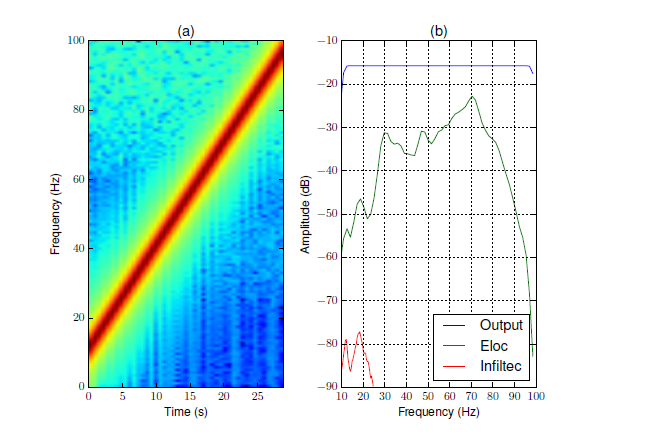
\includegraphics[width=10cm,height=13cm,keepaspectratio]{eloc_vs_infiltec.png}
\caption{Sensitivity comparison of the microphones for different
frequencies. The spectrogram (a) shows the played
chirp from 10 Hz to 100 Hz and the graph (b) shows the received
power by an Eloc node and an Infiltec device. Eloc
node is sensitive even to much higher frequencies above the
infrasonic range.}
\label{infiltec:eloc}
\end{figure}

\begin{figure}[H]
\centering
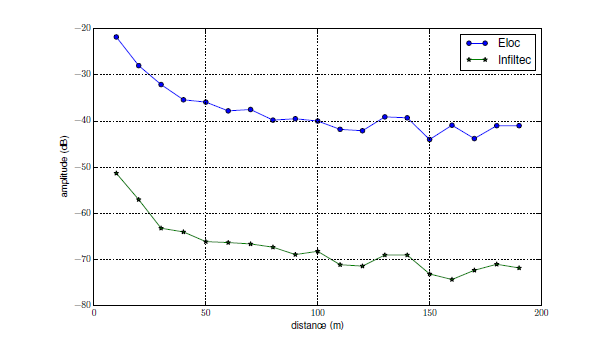
\includegraphics[width=10cm,height=13cm,keepaspectratio]{eloc_vs_infiltec2.png}
\caption{Sensitivity variation of the microphones with distance.
The received power is measured for a 20 Hz tone
for different distances from a subwoofer. Eloc node outperforms
Infiltec device even in longer distances.}
\label{infiltec:eloc2}
\end{figure}

\subsection{Localization experiment 01.}
\paragraph{}
The objective of this experiment was to calibrate our sensors and angle calculating program. This was done in indoor premises placing the speaker 10m away from the sensors and placing the two sensors 3m away from each other. Several recordings were taken by changing the angle between the imaginary line joining two sensors of a infrasonic tone played at 20hz frequency. 

\begin{table}[H]
\centering
\begin{tabular}{|m{0.3\textwidth}|m{0.3\textwidth}|m{0.2\textwidth}|} 
\hline
\bf {Actuale Angle} &  {\bf{ Calculated Angle }} & {\bf{ Difference }}\\
\hline
\hline
\bf {0} &  {\bf{ 1.3058 }} & {\bf{ 1.3058 }}\\
\hline
\bf {30} &  {\bf{ 22.7937 }} & {\bf{ 7.2063 }}\\
\hline
\bf {45} &  {\bf{ 43.7307 }} & {\bf{ 1.2693 }}\\
\hline
\bf {60} &  {\bf{ 51.9516 }} & {\bf{ 8.0484 }}\\
\hline
\bf {90} &  {\bf{ 72.5378 }} & {\bf{ 17.4622 }}\\
\hline
\end{tabular}
\end{table}

\subsection{Localization experiment 02.}

\paragraph{}
After correcting some errors in the angle calculating program and modification of the gain in the sensors, the next experiment was conducted outdoors at the university grounds.  Similar to the indoor experiment, a low frequency was played from a specific position of the ground and recordings were taken from different places of the university.  Before calculating the angles, FFT was applied to the signals and frequency against sample count was plotted, to check whether the played tone is received by the microphones. FFT graph of some of the audio clips are shown below. The frequency of the played wave during the experiment was 20Hz.


\paragraph{}
These angles were calculated by considering several windows from the recorded audio and the mode of the angles calculated in different windows were considered in this initial experiment.

\begin{figure}[H]
\centering

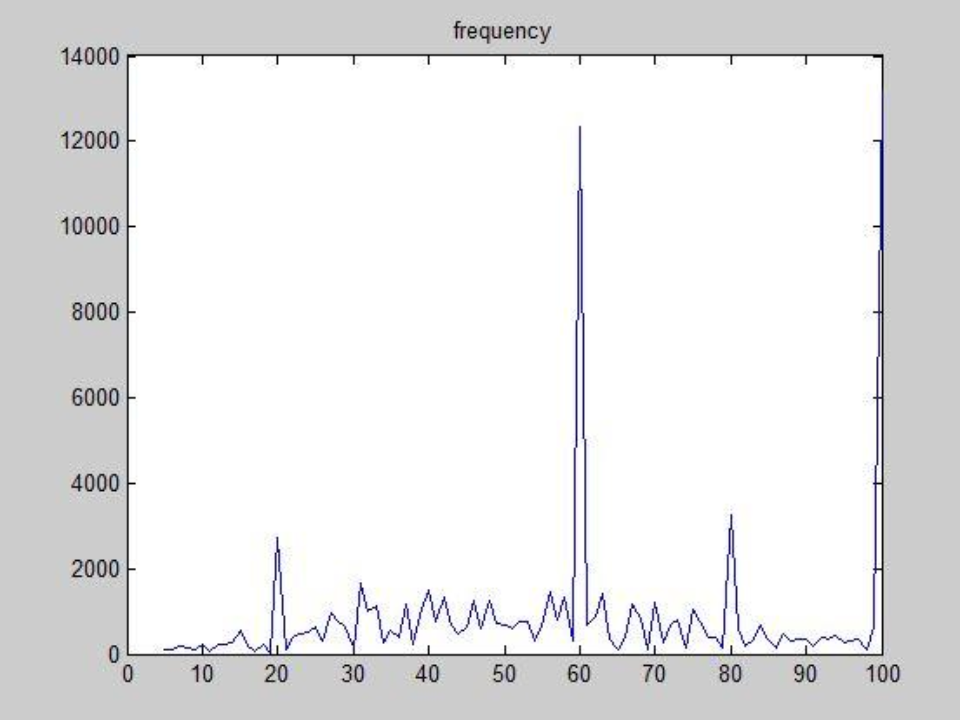
\includegraphics[width=10cm,height=13cm,keepaspectratio]{position3.png}
\caption{FFT at position 3}
\label{d:p3}
\end{figure}

\begin{figure}[H]
\centering
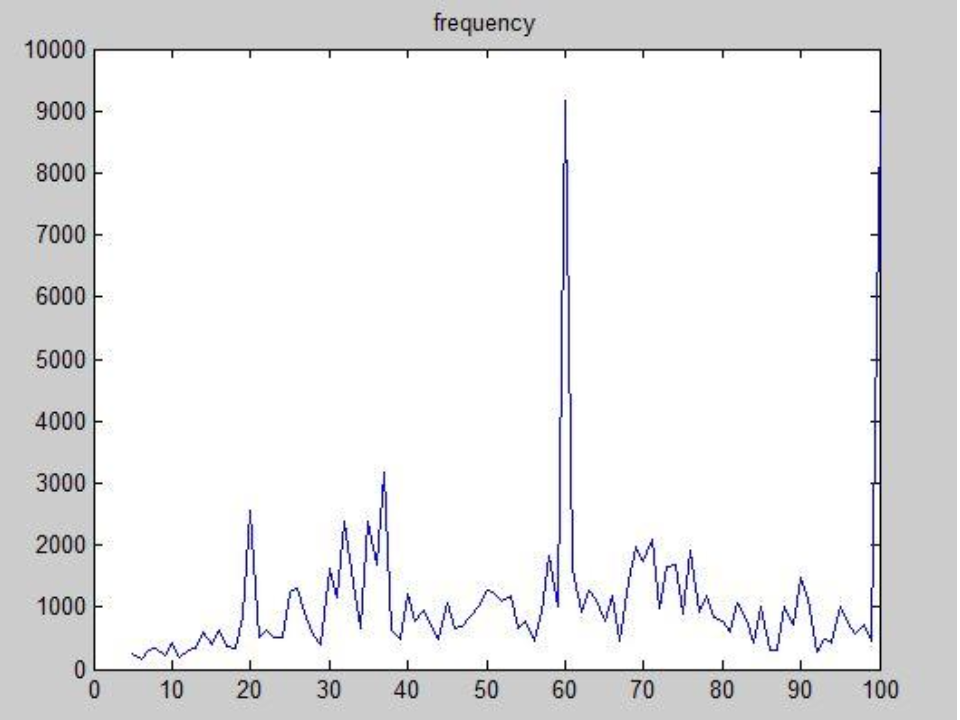
\includegraphics[width=10cm,height=13cm,keepaspectratio]{position7.png}
\caption{FFT at position 7}
\label{d:p7}
\end{figure}

\paragraph{}
By looking at the above graphs, it is clear that the infrasonic waves reached two of the furthest recording places away from the speaker. Figure \ref{d:map} show the locations of the places where recordings were done.

\begin{figure}[H]
\centering
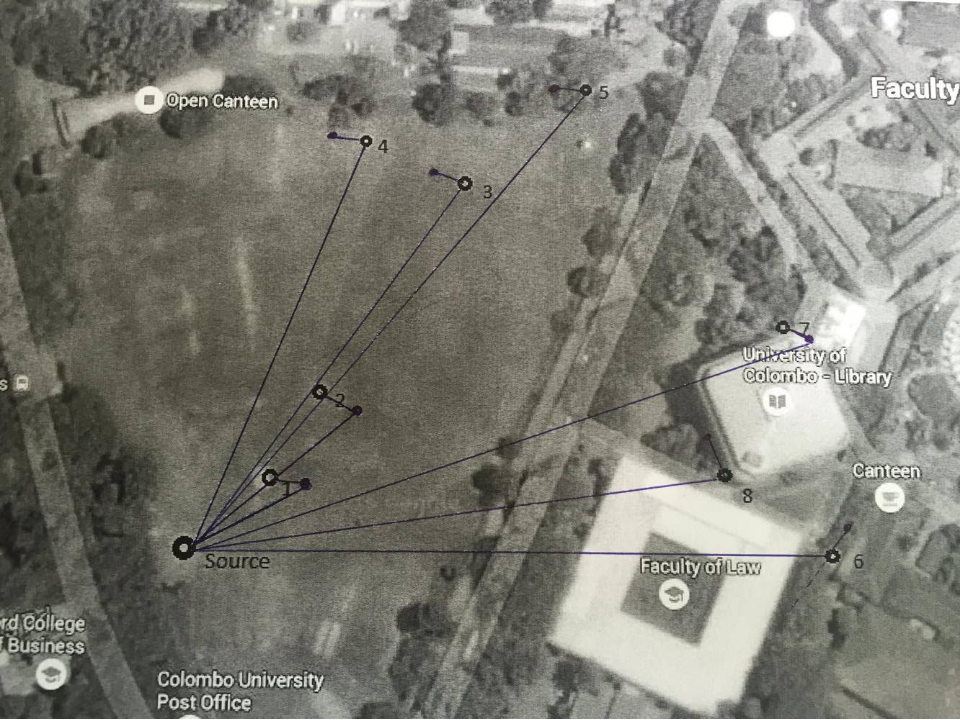
\includegraphics[width=14cm,height=11cm,keepaspectratio]{map.png}
\caption{Recording locations}
\label{d:map}
\end{figure}

\paragraph{}
The estimated angle and actual angles of each positions can be found in the following table. Note that the actual angles are estimated geometrically using Google map.

\begin{table}[H]
\centering
\begin{tabular}{|m{0.3\textwidth}|m{0.3\textwidth}|m{0.2\textwidth}|} 
\hline
\bf {Actuale Angle} &  {\bf{ Calculated Angle }} & {\bf{ Difference }}\\
\hline
\hline
\bf {30} &  {\bf{ 25.209  }} & {\bf{ +4.791 }}\\
\hline
\bf {60} &  {\bf{ 59.574 }} & {\bf{ +0.426 }}\\
\hline
\bf {50} &  {\bf{ 48.457 }} & {\bf{ +1.543 }}\\
\hline
\bf {55} &  {\bf{ 59.909 }} & {\bf{ -4.909 }}\\
\hline
\bf {45} &  {\bf{ 45.153 }} & {\bf{ -0.153 }}\\
\hline
\bf {70} &  {\bf{ 65.692 }} & {\bf{ +4.308 }}\\
\hline
\bf {30} &  {\bf{ 26.912 }} & {\bf{ +3.088 }}\\
\hline
\end{tabular}
\end{table}

\newpage
\subsection{Localization experiment 03.}

\paragraph{}
In this experiment, instead of taking out the mod value of the angles calculated in different windows, we plotted the histogram of the angle distribution. Similar to the above experiment, the sound source was placed at the same location and recordings were taken at different angles between the source and the sensors. This time, actual angles were calculated geometrically at the location using basic simple geometric construction theories. The following table shows the results related to the experiment.


\begin{figure}[H]
  \centering
  \begin{minipage}[b]{0.4\textwidth}
    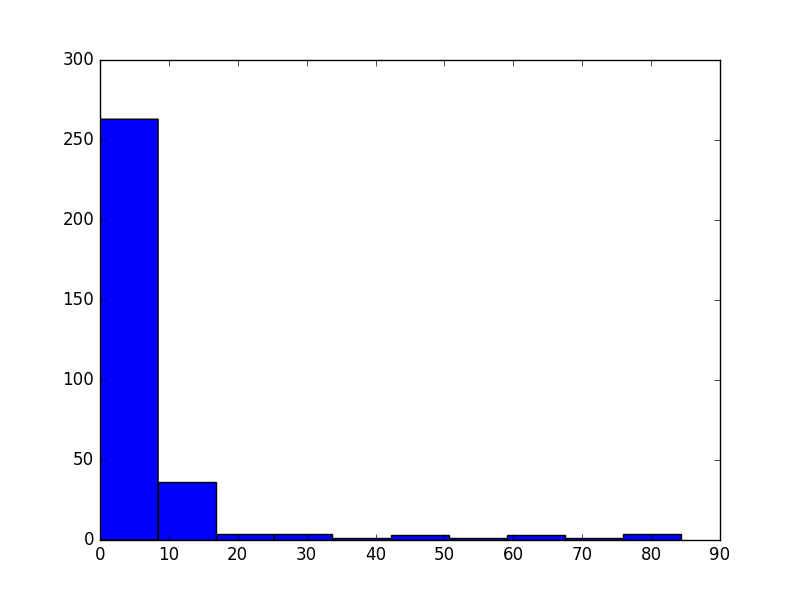
\includegraphics[width=\textwidth]{figure_1.png}
    \caption{0 degree histogram.}
  \end{minipage}
  \hfill
  \begin{minipage}[b]{0.4\textwidth}
    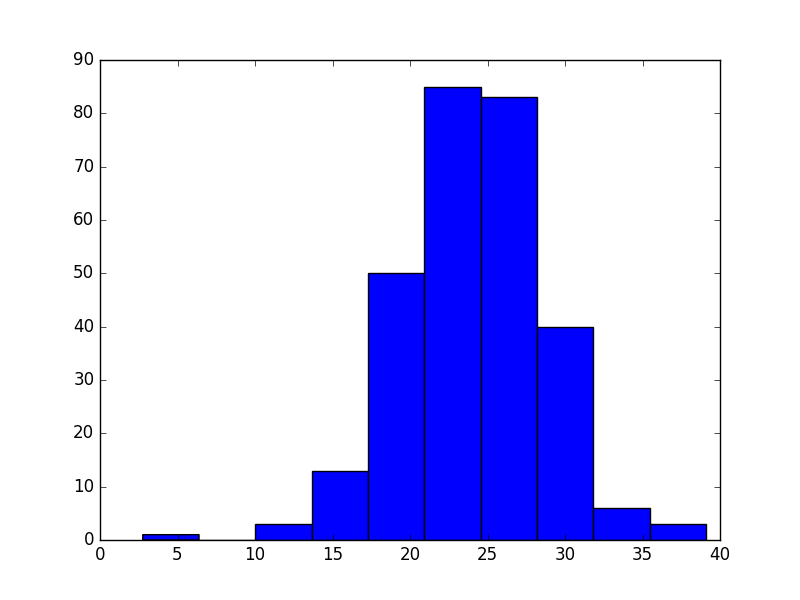
\includegraphics[width=\textwidth]{figure_20.png}
    \caption{20 degree histogram}
  \end{minipage}
\end{figure}

\begin{figure}[H]
  \centering
  \begin{minipage}[b]{0.4\textwidth}
    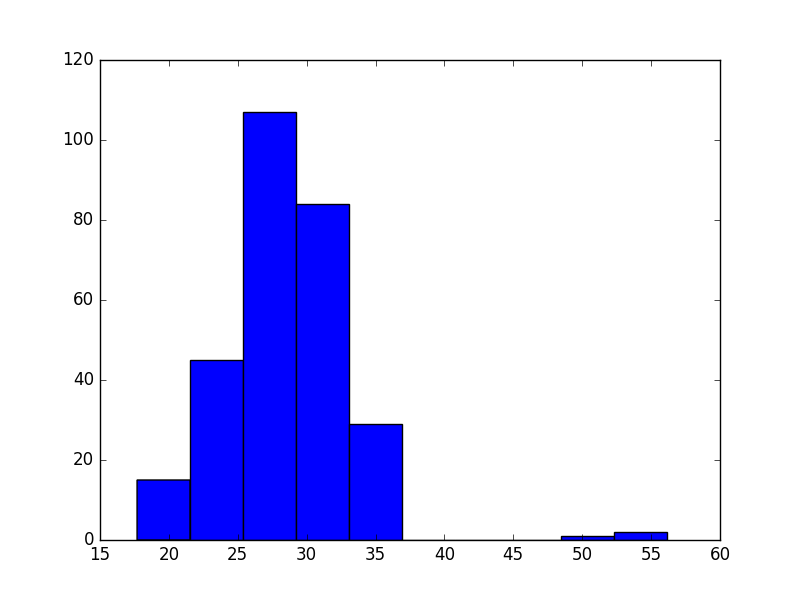
\includegraphics[width=\textwidth]{figure30.png}
    \caption{30 degree histogram.}
  \end{minipage}
  \hfill
  \begin{minipage}[b]{0.4\textwidth}
    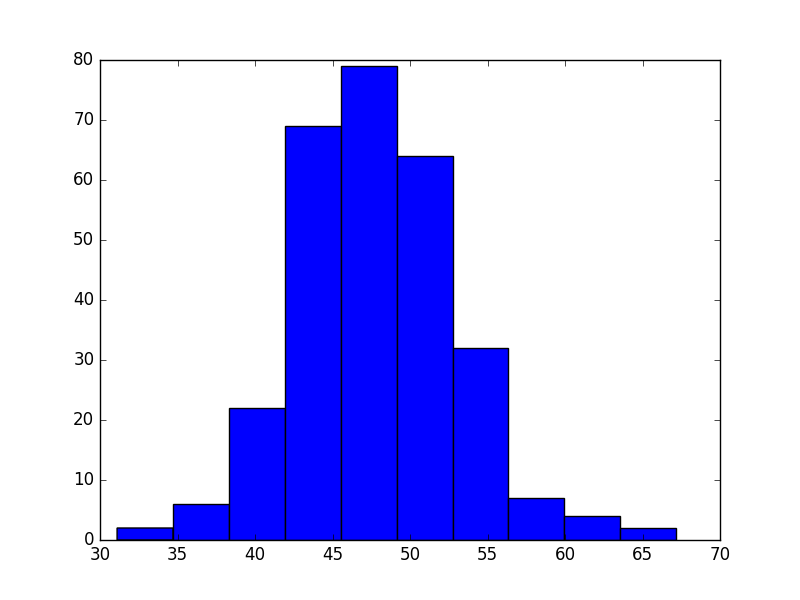
\includegraphics[width=\textwidth]{figure50.png}
    \caption{50 degree histogram}
  \end{minipage}
\end{figure}

\begin{figure}[H]
  \centering
  \begin{minipage}[b]{0.4\textwidth}
    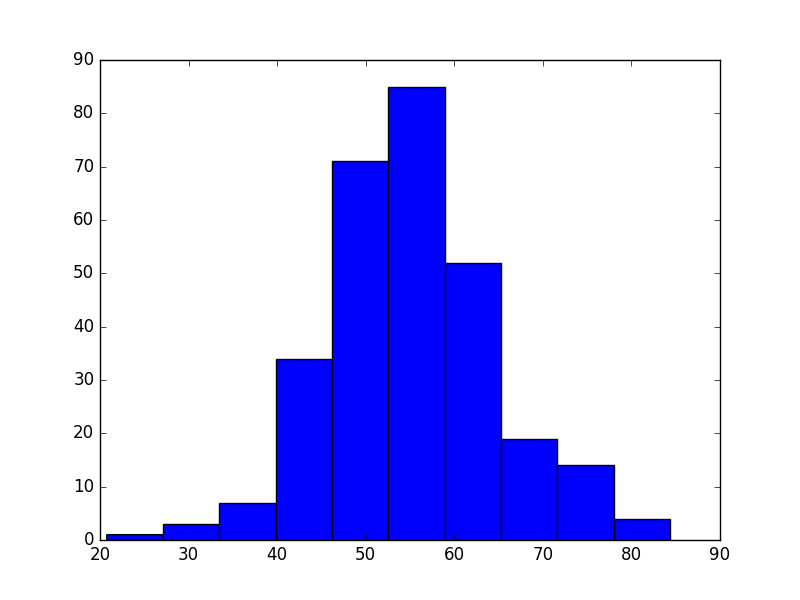
\includegraphics[width=\textwidth]{figure_60.png}
    \caption{60 degree histogram.}
  \end{minipage}
  \hfill
  \begin{minipage}[b]{0.4\textwidth}
    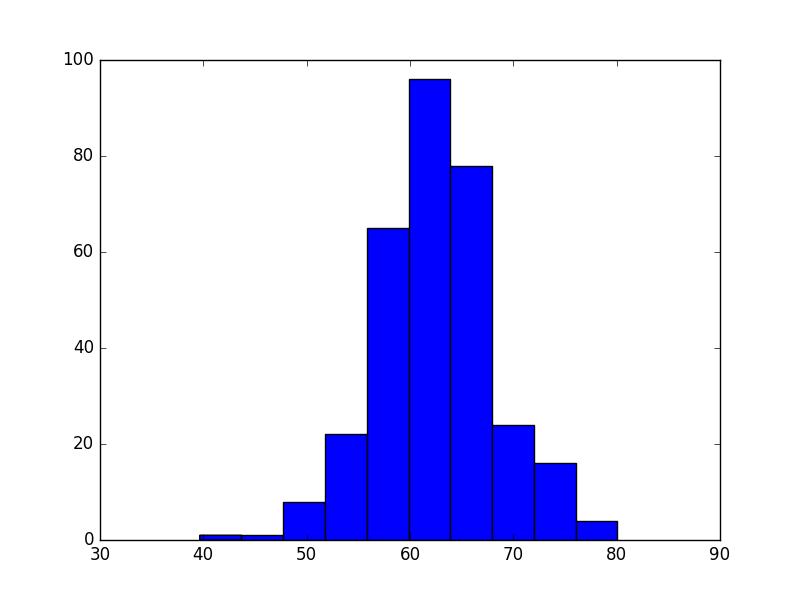
\includegraphics[width=\textwidth]{figure_70.png}
    \caption{70 degree histogram}
  \end{minipage}
\end{figure}

\paragraph{}
Following table shows the number of windows have been produced in the correct range as well as the total number of windows.

\begin{table}[H]
\centering
\begin{tabular}{|m{0.2\textwidth}|m{0.2\textwidth}|m{0.2\textwidth}|m{0.2\textwidth}|} 
\hline
\bf {Actuale Angle} &  {\bf{ Calculated Range }} & {\bf{ Window count }} & {\bf{Total window count}}\\
\hline
\hline
\bf {0} &  {\bf{ 0-7.2  }} & {\bf{250 }} & {\bf{ 402 }}\\
\hline
\bf {10} &  {\bf{ 7.9-11.6 }} & {\bf{85 }} & {\bf{ 345 }}\\
\hline
\bf {20} &  {\bf{ 24.7-27.4 }} & {\bf{65 }} & {\bf{ 347 }}\\
\hline
\bf {30} &  {\bf{ 26.4-30.8 }} & {\bf{120 }} & {\bf{ 331 }}\\
\hline
\bf {40} &  {\bf{ 30.8-34.9 }} & {\bf{120 }} & {\bf{ 310 }}\\
\hline
\bf {50} &  {\bf{ 34-41.5 }} & {\bf{100 }} & {\bf{ 332 }}\\
\hline
\bf {60} &  {\bf{ 46-50}} & {\bf{ 110}} & {\bf{ 460 }}\\
\hline
\bf {70} &  {\bf{ 53-62 }} & {\bf{ 55 }} & {\bf{ 366}}\\
\hline
\bf {80} &  {\bf{ 65-69 }} & {\bf{ 110 }} & {\bf{ 431 }}\\
\hline
\bf {90} &  {\bf{ 65-79 }} & {\bf{ 110 }} & {\bf{ 384}}\\
\hline
\bf {90} &  {\bf{ 70-73 }} & {\bf{ 90 }} & {\bf{ 507}}\\
\hline
\end{tabular}
\end{table}


\paragraph{}
We can observe that when angles get close to 90 degrees, the total error gradually increases. The next phase of the localization experiment is to heuristically find an angle with a minimum error or defining the factors affecting the error and using those factors building an equation for the angle error.
\paragraph{}
Apart from the localization experiments, there were few attempts to record vocals of the wild elephants in Sri Lanka at Kalawewa and Yala. During the visit to Kalawewa, the recordings were done in the presence of an elephant herd and a total hour of 8 was recorded. All visible and audible behavior of the elephants were recorded. Thereafter, these data were successfully backed up and logged in a digital spreadsheet. 
\paragraph{}
During the visit to Yala, we were able to place the sensors, so that recorded data could also be used for the purpose of localization. There were few significant incidents during the visit and the analyzed results of a recorded audio at one such instance is shown in the following figure.

\begin{figure}[H]
\centering
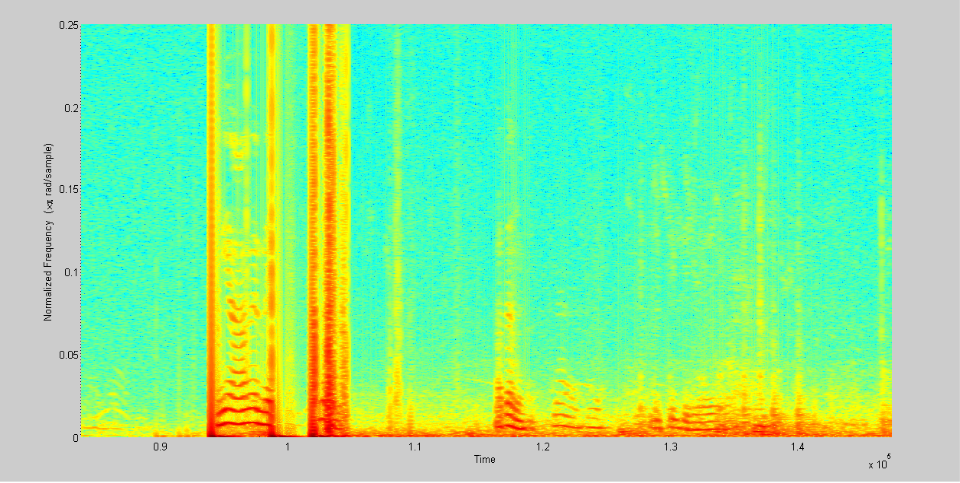
\includegraphics[width=14cm,height=11cm,keepaspectratio]{44100.png}
\caption{Spectogram of the signal under 44100 sample rate}
\label{d:44100}
\end{figure}

The above image shows the spectrogram of a recorded clip at a sample rate of 44100 . The patterns of elephant rumbles are shown by the small red curves \cite {19}. If the above clip re-sampled at sample rate of 250 , the infrasonic rumble patterns become visible.

\begin{figure}[H]
\centering
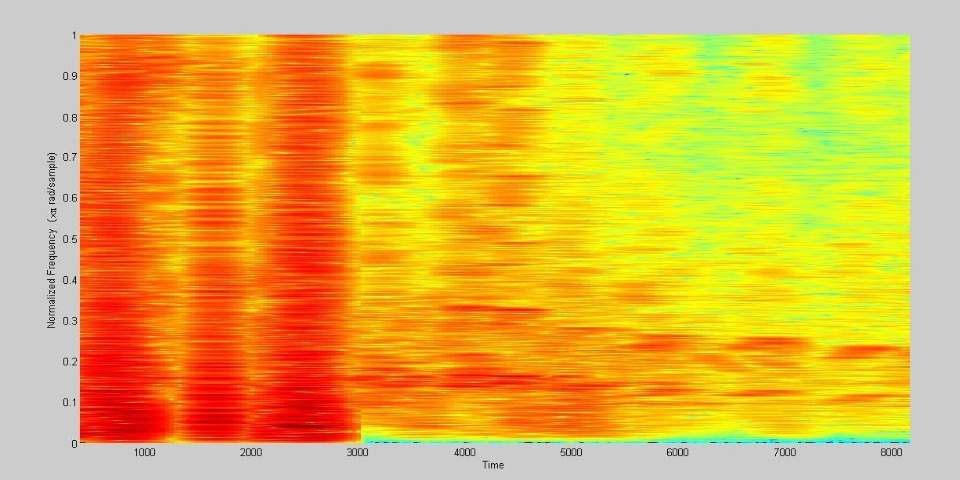
\includegraphics[width=14cm,height=11cm,keepaspectratio]{200.png}
\caption{Spectogram of the signal under 200 sample rate}
\label{d:200}
\end{figure}

\paragraph{}
As this was recorded by the localizable configurations of the devices, this signal can also be analyzed to calculate angles of the elephant location. Some clips where rumbles are visible, were cropped using the spectrogram. These clips are cropped one after the other, so that it indicates the rumbles of the moving elephant herd. Estimated angle ranges from the plotted histograms are shown below.

\begin{table}[H]
\centering
\begin{tabular}{|m{0.5\textwidth}|m{0.3\textwidth}|} 
\hline
\bf {Clip} &  {\bf{Angle range}}\\
\hline
\hline
\bf {160402001Mcropped1.wav } &  {\bf{ 40-45  }} \\
\hline
\bf {160402001Mcropped2.wav } &  {\bf{47-50}} \\
\hline
\bf {160402001Mcropped3.wav} &  {\bf{  54-56}} \\
\hline
\bf {160402001Mcropped4.wav} &  {\bf{ 55-57 }} \\
\hline
\bf {160402001Mcropped5.wav } &  {\bf{  50-60   (a rather longer clip) }} \\
\hline
\bf {160402001Mcropped6.wav} &  {\bf{ 55-60}} \\
\hline
\end{tabular}
\end{table}

\newpage
\subsection{Error and correction of the angle}
\begin{figure}[H]
\centering
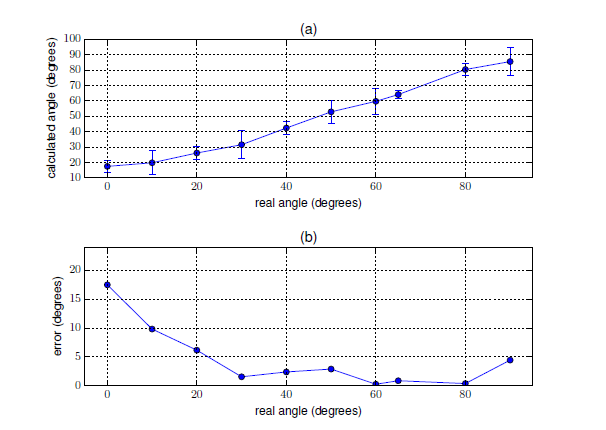
\includegraphics[width=10cm,height=13cm,keepaspectratio]{error_angles.png}
\caption{Accuracy of calculating the direction to an infrasonic
source using a pair of Eloc nodes. The figure’s top
part shows the relationship between real angles and respective
calculated angles. The lower part shows the variation of
the error in calculation against the real angle in consideration.
For angles above 30 degrees the error is low.}
\label{d:p7}
\end{figure}


\subsection{Elephant Sound Recording in the Wild}

\paragraph{}
The previous experiment confirms that Eloc nodes together with the wind shield can identify infrasonic frequencies inside the controlled environment of a laboratory even when there is wind. However, real deployments pose further challenges such as vehicle noise from nearby areas, vibrations that occur on the Eloc nodes due to the impact of dust and vegetation in the deployed location. Therefore, we evaluate the effectiveness of Eloc nodes to identify low frequency elephant sounds in the wild.
\paragraph{}
In order to capture real elephant sounds, we take a
pair of Eloc nodes to a national park in Country where free
ranging elephants live. We mount the nodes inside an offroad
vehicle and park it in a location inside the national park
where we can observe elephants visually while recording
sounds. The vehicle engine is turned off during the recording
time. Other external noise sources such as wind and vehicles
in the nearby areas are present. We note the presence of elephants
and their behavior in the visual range and compare
them against the data we record. We take support of a zoologist
to verify whether the recorded patterns are from an
elephant
\paragraph{}
Figure 5.13 illustrates the waveform, frequency domain and the spectrogram of an elephant sound identified by
a zoologist from our field recordings. As the figure shows, Eloc nodes can clearly capture the fundamental frequency
component of the sound that is below the 25 Hz in addition to the higher frequency harmonics. However, due to the effect
of the low-pass filter in Eloc nodes, the frequencies above 150 Hz are significantly attenuated.

\begin{figure}[H]
\centering
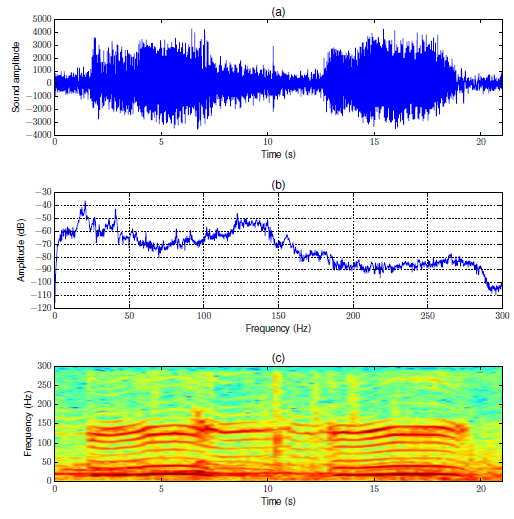
\includegraphics[width=10cm,height=13cm,keepaspectratio]{wild_recordings.png}
\caption{An excerpt from the elephant sound recordings using
a pair of Eloc nodes. The graph (a) shows the waveform
of the signal while the graph (b) shows its frequency domain.
Graph (c) illustrates the spectrogram of the signal where a
number of higher harmonics of the fundamental frequency of
the elephant sound is visible. (The waveform shown in graph
(a) has the amplitude as a scalar value between +215 and
+215 since we store the recorded data in wave files which
uses 16-bit Pulse Code Modulation (PCM))}
\label{d:p7}
\end{figure}

\subsection{Elephant detection model}
\subsubsection{Data set}
\subsubsection{Accuracy}
\subsubsection{Improvements}

\newpage
\section{Conclusion and Future Works.}
\begin{itemize}
  \item New possibilities discovered.
  \item Problems encountered.
  \item Increasing the accuracy of detection and localization.
  \item Summary
\end{itemize}

\newpage
\begin{thebibliography}{1}
\bibitem{1} Berg, J.K. 1983. Vocalizations and associated behaviours of the African elephant Loxodonta africana in captivity. Z. Tierpsychol 63:63-79.
\bibitem{2}Payne, K. 2003. Sources of Social Complexity in the Three Elephant Species. In: Animal Social Complexity: Intelligence, Culture, and Individualized Societies. Ed: Frans B.M. de Waal and Peter L. Tyack. Harvard University Press.
\bibitem{3} Payne, K., Langbauer, Jr., W.R., and Thomas, E. 1986. Infrasonic calls of the Asian elephant (Elephas maximus). Behavioral Ecology and Sociobiology.
\bibitem{4} “Infrasonic Sound", Hyperphysics.phy-astr.gsu.edu, 2016. [Online]. Available: http://hyperphysics.phy-astr.gsu.edu/hbase/sound/infrasound.html. [Accessed: 27- Apr- 2016].
\bibitem{5} Szabo T. L., 1994, “Time domain wave equations for lossy media obeying a frequency power law,” J. Acoust. Soc. Am., 96(1), pp. 491-500.
\bibitem{6} Payne, K., Thompson, M., and Kramer, L. 2003. Elephant calling patterns as indicators of group size and composition: the basis for an acoustic monitoring system. African Journal of Ecology, 41: 99-107
\bibitem{7} "INFILTEC: The Inexpensive Infrasound Monitor Project. - simple microbarograph design for DIY", Infiltec.com, 2016. [Online]. Available: http://www.infiltec.com/Infrasound@home/. [Accessed: 27- Apr- 2016].
\bibitem{8} A. Vedurmudi, J. Goulet, J. Christensen-Dalsgaard, B. Young, R. Williams and J. van Hemmen, "How Internally Coupled Ears Generate Temporal and Amplitude Cues for Sound Localization",Phys. Rev. Lett., vol. 116, no. 2, 2016.
\bibitem{9} ] Larom, D., M. Garstang, K. Payne, R. Raspet \& M. Lindeque. 1997. The influence of surface atmospheric conditions on the range and area reached by animal vocalizations. J. Experimental Biol. 200: 421-431.
\bibitem{10} P. J. Venter and J. J. Hanekom. Automatic detection of african elephant (loxodonta africana) infrasonic vocalisations from recordings. Biosystems engineering.
\bibitem{11} Acoustic Detection of Elephant Presence in Noisy Environments Matthias Zeppelzauer Vienna University of Technology.
\bibitem{12} MUSIC Algorithm", Ptolemy.eecs.berkeley.edu, 2016. [Online]. Available: http://ptolemy.eecs.berkeley.edu/papers/96/dtmf\_ict/www/node5.html. [Accessed: 27- Apr- 2016].
\bibitem{13} Lalith Seneviratne, G. Rossel, W.D.C.. Gunasekera, H.L.P.A. Madanayake, Y.M.S.S. Yapa and G. Doluweera.Elephant Infrasound Calls as a Method for Electronic Elephant Detection.
\bibitem{14} J. E. Piercy, T. F. W. Embleton, L. C. Sutherland, Review of noise propagation in the atmosphere, J. Acoust. Soc. Am. Volume 61, Issue 6, pp. 1403-1418, June 1977.
\bibitem{15} Panasonic Corporation. Panasonic Omnidirectional Back Electret Condenser Microphone Cartidge.[2016].  [Online]. Available: http://industrial.panasonic.com/cdbs/www-data/pdf/ABA5000/ABA5000CE22.pdf. [Accessed: 28- Apr- 2016].
\bibitem{16}"LM358 | General Purpose Amplifier | Operational Amplifier (Op Amp) | Description \& parametrics", Ti.com, 2016. [Online]. Available: http://www.ti.com/product/LM358. [Accessed: 28- Apr- 2016].
\bibitem{17}Jean-Marc Valin, Franc¸ois Michaud, Jean Rouat, Dominic Letourneau LABORIUS - Research Laboratory on Mobile Robotics and Intelligent Systems Department of Electrical Engineering and Computer Engineering Universite´ de Sherbrooke.Robust Sound Source Localization Using a Microphone Array on a Mobile Robot.
\bibitem{18} Richard F. Lyon, Andreas G. Katsiamis, Emmanuel M. Drakakis (2010). "History and Future of Auditory Filter Models"
\bibitem{19} Shermin de Silva "Acoustic communication in the Asian elephant,
Elephas maximus maximus"
\bibitem{20} Taff, L. G, “Target Localization from Bearings-only Observations,”
IEEE Trans. Aerosp. Electron., 3, issue 1, (1997).New York: McGraw-Hill, 1964, pp. 15–64.
\bibitem{21}D.Li, and Y. H. Hu, “Energy Based Collaborative Source Localization
Using Acoustic Micro-Sensor Array,” EURASIP Journal on Applied
Signal Processing, vol. 2003, no. 4, pp. 321-337, 2003.
\bibitem{22}M. Brandstein and H. Silverman, “A Practical Methodology for Speech
Source Localization with Microphone arrays,” Comput., Speech Lng.,
vol. 11, no. 2, pp. 91-126, 1997.
\bibitem{23} G. C. Carter, “Tutorial Overview of Coherence and Time Delay Estimation,”
in Coherence and Time Delay Estimation—An Applied Tutorial for Research, Development, Test, and Evaluation Engineers, vol. 1,1993,pp. 1–27
\bibitem{24}C. H. Knapp and G. C. Carter, “The Generalized Correlation Method for Estimation of Time Delay,” IEEE Trans. Acoust., Speech, Signal Processing,vol. ASSP-24, pp. 320–327, Aug.1976.
\bibitem{25}  J.benesty, “Adaptive Eigenvalue Decomposition Algorithm for Passive Acoustic Source Localization,” Acoustical Society of America, January 2000.
\bibitem{26} Hasan Khaddour, "A Comparison of Algorithms of Sound Source Localization Based
on Time Delay Estimation"
\bibitem{27} Sasha Devore,Antje Ihlefeld,Kenneth Hancock,Barbara Shinn-Cunningham,Bertrand Delgutte,
"Accurate Sound Localization in Reverberant Environments Is Mediated by Robust Encoding of Spatial Cues in the Auditory Midbrain"
\bibitem{28}M.P.J. Dharmaratne and P.C. Magedaragamage, Human-Elephant conflict and solutions to it in Sri Lanka.
\bibitem{29} Infiltec Model INFRA-20 the inexpensive infrasound monitor device. http://www.infiltec.com/Infrasound@home/. Accessed: 2015-07-29.
\bibitem{30} K. B. Payne, J. W. R. Langbauer, and E. M. Thomas. Infrasonic calls of the asian elephant (elephas maximus). Behavioral Ecology and Sociobiology, 18(4):297–301, 1986.
\bibitem{31}P. Dabare, C. Suduwella, A. Sayakkara, D. Sandaruwan, C. Keppitiyagama, K. De Zoysa, K. Hewage, and T. Voigt. Listening to the giants: Using elephant infra-sound to solve the human-elephant conflict. In Proceedings of the 6th ACMWorkshop on RealWorldWireless Sensor Networks, pages 23–26. ACM, 2015.
\bibitem{32} S. Blake, I. Douglas-Hamilton, andW. Karesh. Gps telemetry of forest elephants in central africa: results of a preliminary study. African Journal of Ecology, 39(2):178–186, 2001.
\bibitem{33}H. Wang, C.-E. Chen, A. Ali, S. Asgari, R. E. Hudson, K. Yao, D. Estrin, and C. Taylor. Acoustic sensor networks for woodpecker localization. In Optics Photonics 2005, pages 591009–591009. International Society for Optics and Photonics, 2005.
\bibitem{34}Y.-E. Kim, C.-H. Jeon, D.-H. Su, J.-K. Lee, J.-G. Chung, and K.-J. Cho. Sound Source Localization Method Using Region Selection.INTECH Open Access Publisher, 2011.
\bibitem{35}J. Taylor. Introduction to Error Analysis, the Study of Uncertainties in Physical Measurements, 2nd Edition. University Science Books, Aug.1997.

\end{thebibliography}

\end{document}